%%%%%%%%%%%%%%%%%%%%%%%%%%%%%%%%%%%%%%%%%%%%%%%%%%%%%%%%%%%%%%%%%%%%%%%%%%%%%%
\documentclass[aspectratio=169]{beamer}            % Generate slides
%\documentclass[handout]{beamer}   % Generate handouts (6 slides to 1 page)
%\documentclass[aspectratio=169]{beamer}  % Use widescreen 16:9 aspect ratio
    % Possible aspect ratios are 16:9, 16:10, 14:9, 5:4, 4:3 (default) and 3:2
    % (Remember to remove the colon)

\usetheme{UoB}
%\usetheme[compress]{UoB}     % Compress the margins
%\usetheme[nourl]{UoB}        % Remove the footer with the URL
%\usetheme[nowatermark]{UoB}  % Remove the watermark from the title page

% Generate handouts with notes (3 slides + 3 notes to 1 page)
%\mode<handout>{
%  \pgfpagesuselayout{3 on 1 with notes}[a4paper,border shrink=10mm]
%}

\usepackage{nomencl} % nomenclature generation via makeindex
	\makenomenclature
\usepackage{tikz}
\usetikzlibrary{matrix,chains,scopes,arrows,positioning,fit,
	decorations.pathmorphing,decorations.markings,shapes,calc}
\usepackage[binary-units = true]{siunitx}
\usepackage{subfig}

\usepackage{pgfplots}
\pgfplotsset{compat=1.15}

\usepackage{multimedia}

\everymath{\displaystyle}

\graphicspath{{./Figures/}}

%%%%%%%%%%%%%%%%%%%%%%%%%%%%%%%%%%%%%%%%%%%%%%%%%%%%%%%%%%%%%%%%%%%%%%%%%%%%%%
\title[Bio-Inspired Distributed Sensing]{Bio-Inspired Distributed Sensing for
	Improved Flight Control}
%\subtitle{Subtitle}
\author{Sergio A. Araujo-Estrada}
\institute{Research Associate \\
	Aerospace Engineering Department \\
	\href{mailto:s.araujoestrada@bristol.ac.uk}{s.araujoestrada@bristol.ac.uk}}
\date{Thursday, May 3}

%%%%%%%%%%%%%%%%%%%%%%%%%%%%%%%%%%%%%%%%%%%%%%%%%%%%%%%%%%%%%%%%%%%%%%%%%%%%%%
\begin{document}

\setbeamercovered{transparent}

\titlepage

%%%%%%%%%%%%%%%%%%%%%%%%%%%%%%%%%%%%%%%%%%%%%%%%%%%%%%%%%%%%%%%%%%%%%%%%%%%%%%
\begin{frame}{Overview}
	\tableofcontents
\end{frame}

%%%%%%%%%%%%%%%%%%%%%%%%%%%%%%%%%%%%%%%%%%%%%%%%%%%%%%%%%%%%
\section{Introduction}
\subsection{Motivation}
\begin{frame}{Motivation: Why Bio-Inspired Distributed Sensing?}
  
	\pause
  \begin{columns}
    \begin{column}{0.5\textwidth}
      \begin{itemize}
	\item<1->{Current UAV autopilot technologies}
	\item<3->{Challenges}
	\item<5->{Potential use of force and flow information}
      \end{itemize}
    \end{column}
    \begin{column}{0.5\textwidth}  %%<--- here
      \only<2>{
	\begin{itemize}
	  \item[-]{Inertial}
	  \item[-]{Single point air speed}
	  \item[-]{GPS}
	  \item[-]{Vision}
	\end{itemize}
      }
      \only<4>{
	\begin{itemize}
	  \item[-]Intrinsic nonlinear dynamics
	  \item[-]Classic control strategies limitations
	  \item[-]Limitations of inertial controls
	\end{itemize}	  
      }
      \only<6>{
			Potential applications
	\begin{itemize}
	  \item[-]Availability of aerodynamic variables
	  \begin{itemize}
      \item[${\rightarrow}$]Improved flight dynamics model
      \item[${\rightarrow}$]Stall detection
    \end{itemize}
	  \item[-]Earlier gust detection
		\begin{itemize}
		   \item[${\rightarrow}$]Gust rejection/alleviation
		\end{itemize}
		\item[-]Localised information
		\begin{itemize}
		   \item[${\rightarrow}$]Localised control
			\item[${\rightarrow}$]Load tailoring
    \end{itemize}
		
	  %\item[-]Aeroelastic effects
	  %\item[-]Additional 'hidden' information
	\end{itemize}
      }
    \end{column}
  \end{columns}
  
\end{frame}

%%%%%%%%%%%%%%%%%%%%%%%%%%%%%%%%%%%%%%%%%%%%%%%%%%%%%%%%%%%%
\subsection{Research Problem}
\begin{frame}{Research Problem}
  Use force and flow sensing to improve performance of UAVs flight control systems.\\
  \pause
  To achieve this we aim to:
  \begin{itemize}
    \item<3-> Develop distributed force and flow a sensing system for a small scale fixed wing UAV
    \item<4-> Integrate force and flow sensing into conventional flight control system architecture
    \item<5-> Measure response of systems to controlled and natural turbulence
    \item<6-> Develop advanced reflexive flight control system
  \end{itemize}
\end{frame}

%%%%%%%%%%%%%%%%%%%%%%%%%%%%%%%%%%%%%%%%%%%%%%%%%%%%%%%%%%%%%
%\begin{frame}{The hypothesis (or prediction)}
  %What do you think will happen?
  %
  %Fit strain \& differential pressure sensors
  %Carry out WT experiments
  %Carry out outdoors experiments
  %
  %\begin{itemize}
    %\item AoA, Windspeed aero loads compuation/prediction/estimation
    %\item Characterisation of pressure, strain \& force signals as function of ${\alpha}$, V
      %\& ${\delta_{ail}}$
    %\item Acquisition of training/testing daat sets for ANN for ${\alpha}$, V \&
      %${\delta_{ail}}$ prediction
    %\item Identification of stall characteristic markers in pressure \& strain signals, e.g.
      %frequency, variance
    %\item Acquisition of pressure \& strain characteristic response to change in ${q}$
    %\item Explore pressure \& strain response to conditions similar to perching manoeuvre\
    %\item Emulation of pressure \& strain response to gusts
    %\item Identify pressure \& strain response to varying ${q}$, i.e. ${\dot{q}}$
    %\item Vibration of wing has been observed during and after stall. How does this affect
      %pressure \& strain signals?
    %\item Identify pressure \& strain response to varying ${\delta_{ail}}$, i.e.
      %${\dot{\delta}_{ail}}$
  %\end{itemize}
%\end{frame}

%%%%%%%%%%%%%%%%%%%%%%%%%%%%%%%%%%%%%%%%%%%%%%%%%%%%%%%%%%%%
\section{Research at UoB}
\subsection[Previous Research]{Previous Research}
\begin{frame}{Previous Research at UoB: Strain sensing}

  \begin{columns}
    \begin{column}{0.6\textwidth}
			\only<1,3,6>{
				\begin{figure}[!htb]
	  			\centering
	  			\includegraphics[height=0.45\textwidth]{EasySkyGlider_WTGustTest.eps}
	  			\caption{Strain sensing platform}
	  			\label{Fig:StrainExpPlatform}
				\end{figure}
			}
			\only<2>{
				\begin{figure}[!htb]
	  			\centering
	  			% StrainSensorsInWing.tex
\resizebox{!}{0.45\textwidth}{
	\begin{tikzpicture}
		% Auxiliary objects definition
		\tikzstyle{LabelObject}=[fill=white,rectangle,rounded corners,line width=0.5mm,%
			align=center]
		\tikzstyle{ArrowObject}=[red,line width=0.5mm, -latex]
		% Graphics display
	  \node[anchor=south west,inner sep=0] (image) at (0,0)%
	  {\includegraphics[width=\textwidth,trim= 50mm 0mm 50mm 0mm,clip,angle=180]%
	  	{StrainSensorsInWing.eps}};
	  % Define scope with 'image' dimensions as reference
	  \begin{scope}[x={(image.south east)},y={(image.north west)}]
%			  	\draw[help lines,xstep=.05,ystep=.05] (0,0) grid (1,1);
%			  	\foreach \x in {0,1,...,9} { \node [anchor=north] at (\x/10,0) {0.\x}; }
%			    \foreach \y in {0,1,...,9} { \node [anchor=east] at (0,\y/10) {0.\y}; }
	    %% Auxiliary coordinates
	    \coordinate (L0) at (0.875,0.41);   \coordinate (R0) at (0.050,0.42);
	    \coordinate (L1) at (0.800,0.42);   \coordinate (R1) at (0.125,0.41);
	    \coordinate (L2) at (0.720,0.41);   \coordinate (R2) at (0.200,0.42);
	    \coordinate (L3) at (0.640,0.42);   \coordinate (R3) at (0.280,0.41);
	    \coordinate (L4) at (0.565,0.41);   \coordinate (R4) at (0.360,0.42);
	    \coordinate (L5) at (0.490,0.42);   \coordinate (R5) at (0.440,0.41);
	    %% Labels
	    \draw(0.875,0.25) node[LabelObject] (L0_Label) {${L0}$};
	    \draw(0.800,0.55) node[LabelObject] (L1_Label) {${L1}$};
	    \draw(0.720,0.25) node[LabelObject] (L2_Label) {${L2}$};
	    \draw(0.640,0.55) node[LabelObject] (L3_Label) {${L3}$};
	    \draw(0.565,0.25) node[LabelObject] (L4_Label) {${L4}$};
	    \draw(0.490,0.55) node[LabelObject] (L5_Label) {${L5}$};
	    \draw(0.440,0.25) node[LabelObject] (R5_Label) {${R5}$};
	    \draw(0.360,0.55) node[LabelObject] (R4_Label) {${R4}$};
	    \draw(0.280,0.25) node[LabelObject] (R3_Label) {${R3}$};
	    \draw(0.200,0.55) node[LabelObject] (R2_Label) {${R2}$};
	    \draw(0.125,0.25) node[LabelObject] (R1_Label) {${R1}$};
	    \draw(0.050,0.55) node[LabelObject] (R0_Label) {${R0}$};
	    %% Arrows
			\draw[ArrowObject] (L0_Label.north) -- (L0);
			\draw[ArrowObject] (L1_Label.south) -- (L1);
			\draw[ArrowObject] (L2_Label.north) -- (L2);
			\draw[ArrowObject] (L3_Label.south) -- (L3);
			\draw[ArrowObject] (L4_Label.north) -- (L4);
			\draw[ArrowObject] (L5_Label.south) -- (L5);
			\draw[ArrowObject] (R5_Label.north) -- (R5);
			\draw[ArrowObject] (R4_Label.south) -- (R4);
			\draw[ArrowObject] (R3_Label.north) -- (R3);
			\draw[ArrowObject] (R2_Label.south) -- (R2);
			\draw[ArrowObject] (R1_Label.north) -- (R1);
			\draw[ArrowObject] (R0_Label.south) -- (R0);
	  \end{scope}
	\end{tikzpicture}
}
	  			\caption{Strain sensing platform instrumentation}
	  			\label{Fig:StrainExpPlatformInst}
				\end{figure}
			}
			\only<4>{
        \centering
        \movie[width=0.8\textwidth,externalviewer]{
          \includegraphics[height=0.45\textwidth]{EasySkyGlider_WTGustTest.eps}}
					{./Videos/StrainSensingExperiment_037_SlowDownShort.mp4}
			}
			\only<5>{
        \centering
        \movie[width=0.8\textwidth,externalviewer]{
          \includegraphics[height=0.45\textwidth]{EasySkyGlider_WTGustTest.eps}}
					{./Videos/StrainFeedbackCtrl_GustRejection.mp4}
			}
		\end{column}
		\begin{column}{0.4\textwidth}
			\begin{itemize}
				\item<2-> 12 full-bridge strain gauges and amplifiers distributed along spar of wing
				\item<3-> Wind tunnel characterisation
				\item<4,5-> Closed loop free flight
				\item<6-> Outdoor flight testing
			\end{itemize}
		\end{column}
	\end{columns}

\end{frame}

%%%%%%%%%%%%%%%%%%%%%%%%%%%%%%%%%%%%%%%%%%%%%%%%%%%%%%%%%%%%
\begin{frame}{Previous Research at UoB: Strain sensing}
  What did we learned?
	\pause
    \begin{itemize}[<+->]
      \item Strain signal shows linear response with AoA
      \item Stall markers
      \item Strain-based roll control similar performance to IMU based control
			\item Information not available using IMU: AoA, stall, roll acceleration
    \end{itemize}
\end{frame}

%%%%%%%%%%%%%%%%%%%%%%%%%%%%%%%%%%%%%%%%%%%%%%%%%%%%%%%%%%%%
\begin{frame}{Previous Research at UoB: Pressure sensing}

  \begin{columns}
    \begin{column}{0.6\textwidth}
      \only<1,3,5>{
        \begin{figure}[!htb]
			    \centering
          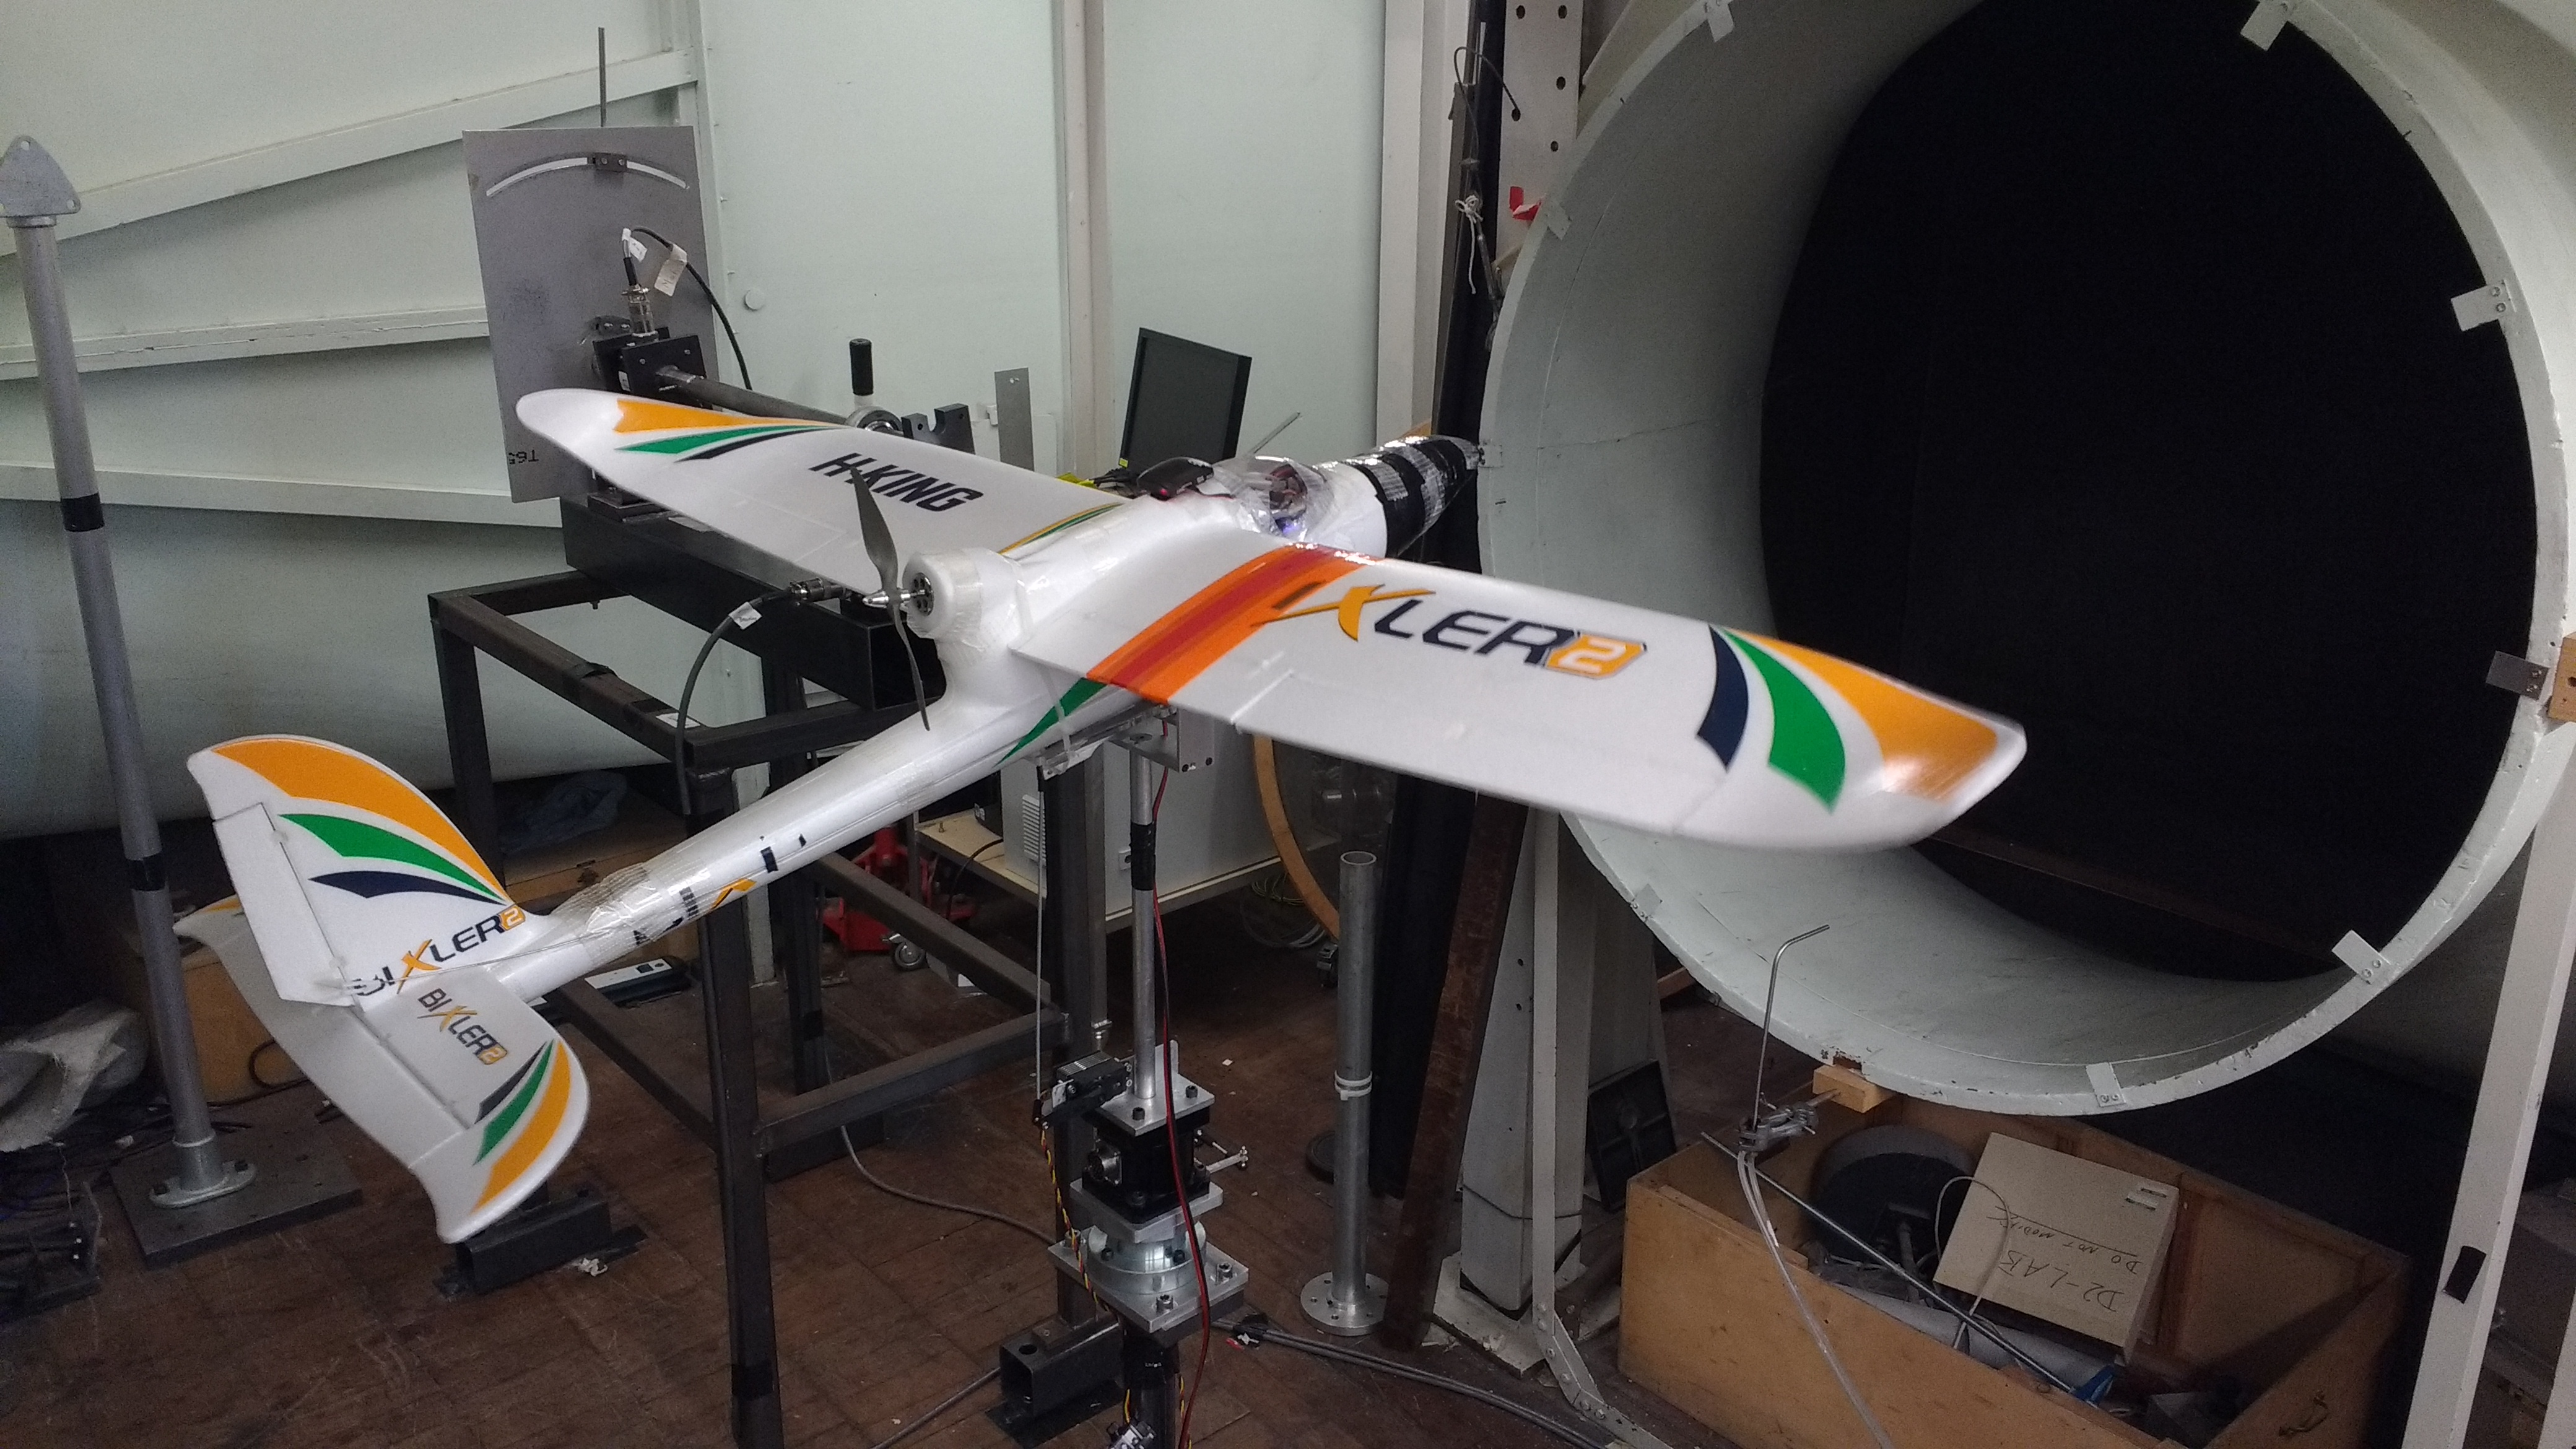
\includegraphics[height=0.45\textwidth]{Bixler_WTTest.eps}
          \caption{Pressure sensing platform}
          \label{Fig:PressureExpPlatform}
        \end{figure}
      }
      \only<2>{
        \begin{figure}[!htb]
          \centering
          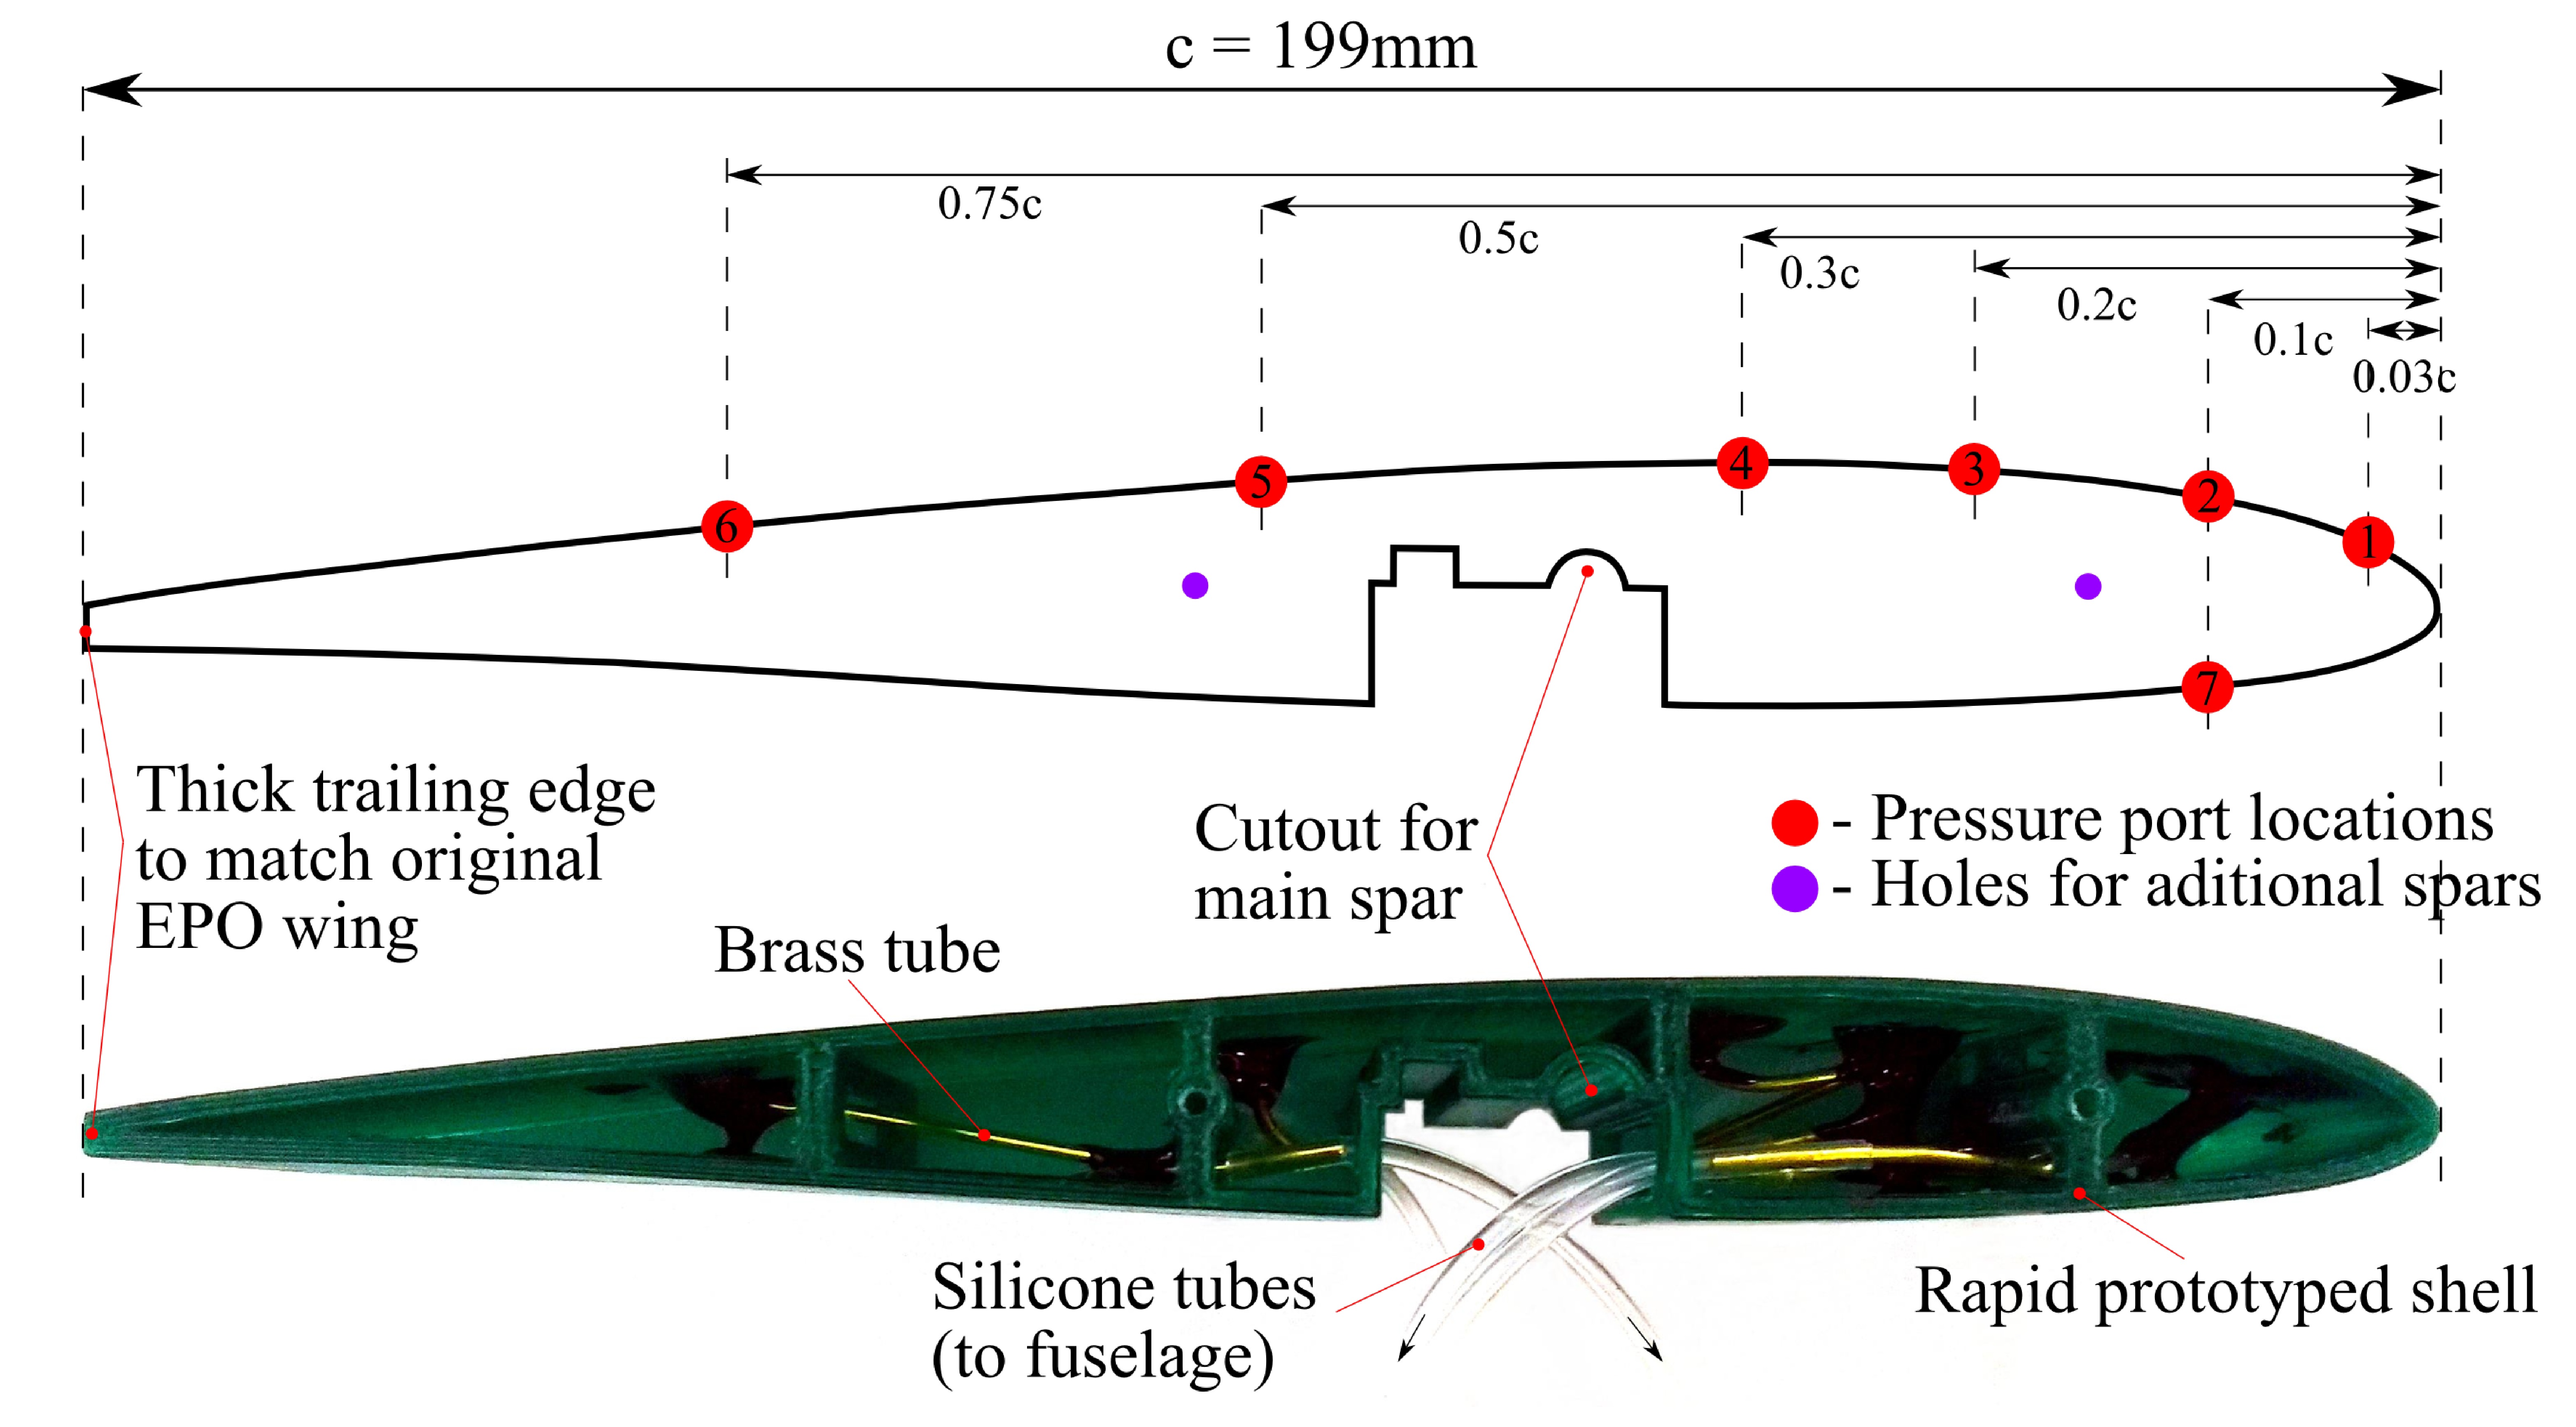
\includegraphics[height=0.45\textwidth]{wingInsertDiagram.eps}
          \caption{Pressure sensing platform instrumentation}
          \label{Fig:PressureExpPlatformInst}
        \end{figure}
      }
			\only<4>{
        \centering
        \movie[width=0.8\textwidth,externalviewer]{
          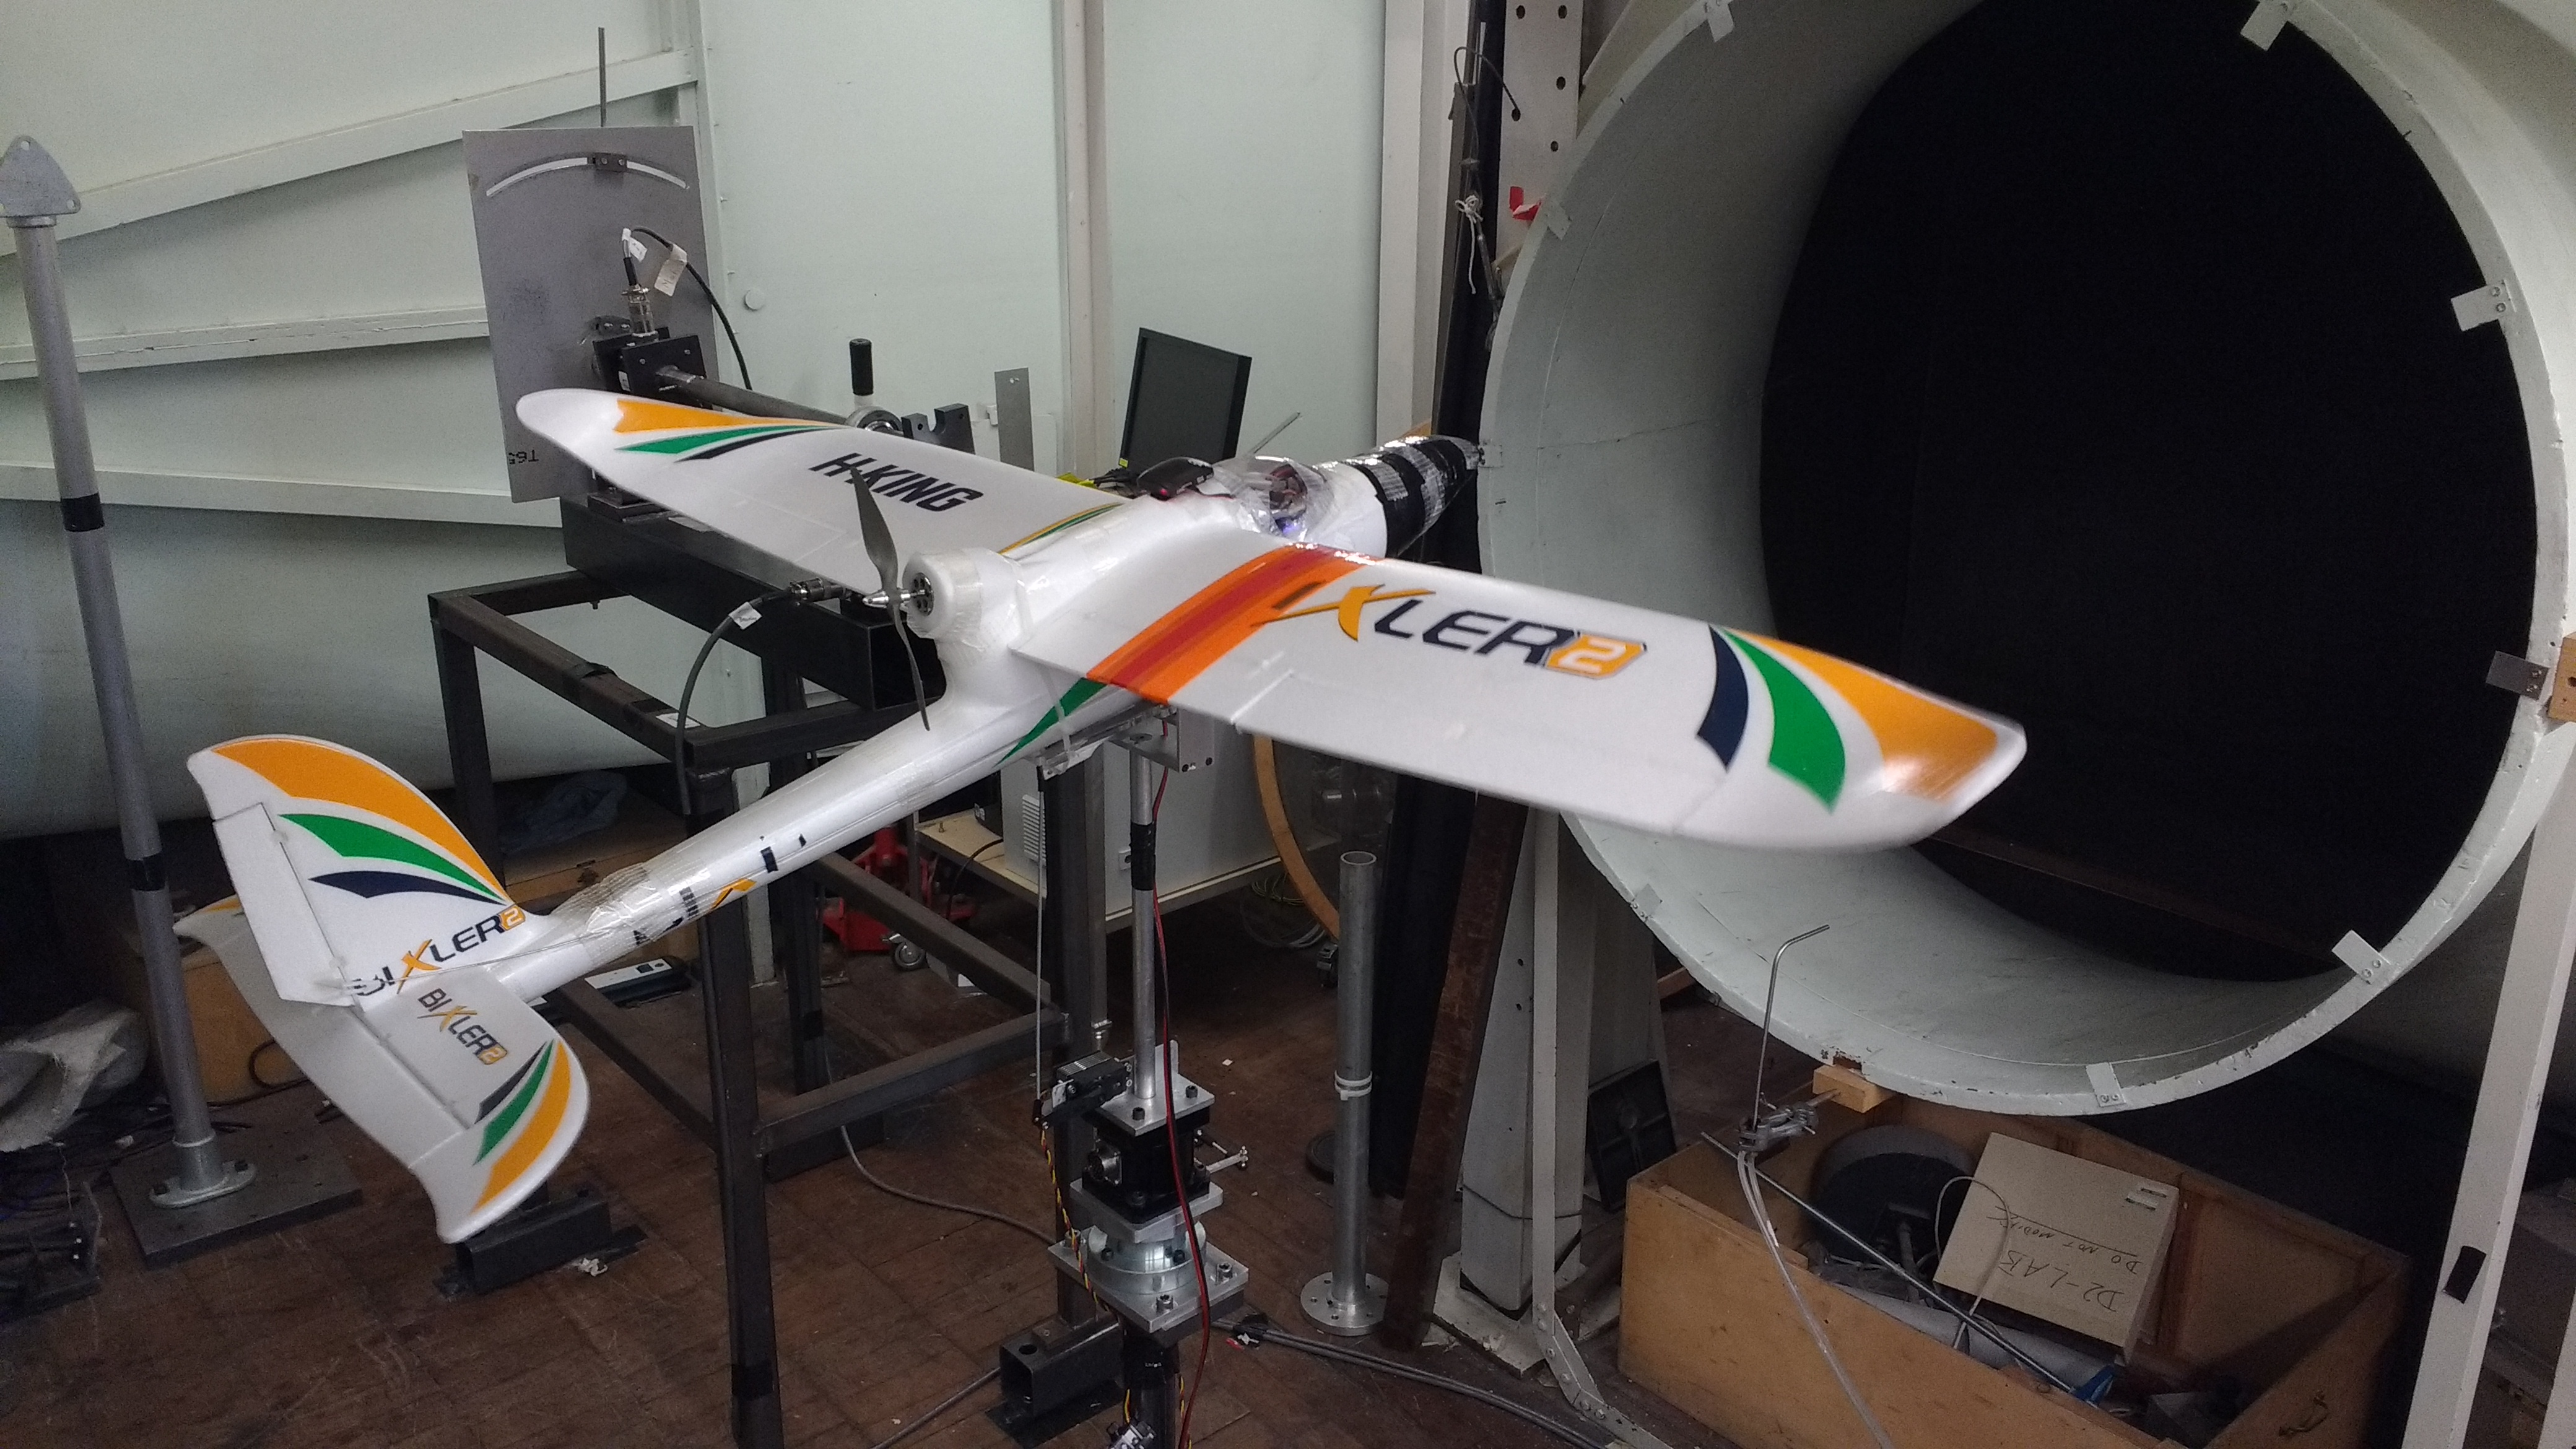
\includegraphics[height=0.45\textwidth]{Bixler_WTTest.eps}}
					{./Videos/WTAoATracking.mp4}
        %\caption{Pressure sensing platform}
			}
		\end{column}
		\begin{column}{0.4\textwidth}
		  \begin{itemize}
				\item<2-> 7 static-pressure ports distributed along wing-chord
				\item<3-> Wind tunnel characterisation
				\item<4-> Closed loop 1DOF WT testing
				\item<5-> Outdoor flight testing
			\end{itemize}
		\end{column}
  \end{columns}
	
\end{frame}

%%%%%%%%%%%%%%%%%%%%%%%%%%%%%%%%%%%%%%%%%%%%%%%%%%%%%%%%%%%%
\begin{frame}{Previous Research at UoB: Pressure sensing}
  What did we learned?
	\pause
    \begin{itemize}[<+->]
      \item Pressure signal shows linear response with AoA
      \item Stall markers
      \item Pitch pressure-based control similar to IMU based control
			\item Information not available using IMU: AoA, stall, non-linear lift
    \end{itemize}
\end{frame}

%%%%%%%%%%%%%%%%%%%%%%%%%%%%%%%%%%%%%%%%%%%%%%%%%%%%%%%%%%%%
\subsection[Current Research]{Current Research}

\begin{frame}{Current Research at UoB}

  \pause
	\begin{itemize}[<+->]
    \item Experimental platform(s) with a distributed array of pressure and strain sensors
    \item Carry out calibration \& characterisation (WT \& outdoors)
    \item Design and implement closed loop control algorithms that use information from distributed array
  \end{itemize}
	\pause
  Divided into two phases:
	\pause
  \begin{itemize}[<+->]
    \item Phase 1: Wind tunnel experiments using WT model
    \item Phase 2: Outdoors experiments using flying platform
  \end{itemize}
  
\end{frame}

%%%%%%%%%%%%%%%%%%%%%%%%%%%%%%%%%%%%%%%%%%%%%%%%%%%%%%%%%%%%
\begin{frame}{Current Research at UoB}

  \begin{columns}
    \begin{column}{0.4\textwidth}
      Wing model instrumentation:
      \pause
      \begin{itemize}
        \item<2->{Chord-wise array of 30 pressure ports in two sections}
        \item<3->{Span-wise array with 16 strain gauges}
				\item<4->{Servo actuated control surfaces}
        \item<6->{MCU-based data acquisition system using, sampling \@ \SI{100}{\hertz}}
        \item<7->{1-DOF pitch motion servo-driven system for automated motion}
      \end{itemize}
    \end{column}
    \begin{column}{0.6\textwidth}
		  \only<2->{
        \begin{figure}[!htb]
          \centering
          % WingSensorDescription.tex

\tikzstyle{RectObject1}=[rectangle,draw=blue,rounded corners,line width=0.5mm,minimum width=3.0em,%
	minimum height=11em]
\tikzstyle{RectObject2}=[rectangle,draw=blue,rounded corners,line width=0.5mm,minimum width=2em,%
	minimum height=2em]
\tikzstyle{RectObject3}=[rectangle,draw=blue,rounded corners,line width=0.5mm,minimum width=3em,%
	minimum height=3em]
\tikzstyle{RectObject4}=[rectangle,draw=blue,rounded corners,line width=0.5mm,minimum width=3.0em,%
	minimum height=4.5em]
\tikzstyle{LabelObject}=[fill=white,rectangle,rounded corners,line width=0.5mm,%
	align=center]
\tikzstyle{ArrowObject}=[red,line width=1.0mm, -latex]

\resizebox{!}{0.4\textwidth}{
	\begin{tikzpicture}
		\node[anchor=south west,inner sep=0] (image) at (0,0)%
			%{\includegraphics[width=\textwidth]{WingSensorDescription.eps}};
			{\includegraphics[width=\textwidth]{WingInstrumentation.eps}};
		% Define scope with 'image' dimensions as reference
		\begin{scope}[x={(image.south east)},y={(image.north west)}]
			%\draw[help lines,xstep=.05,ystep=.05] (0,0) grid (1,1);
			%\foreach \x in {0,1,...,9} { \node [anchor=north] at (\x/10,0) {0.\x}; }
			%\foreach \y in {0,1,...,9} { \node [anchor=east] at (0,\y/10) {0.\y}; }
			
			\only<2>{
			% Pressure Elements
			\draw(0.330,0.475) node[RectObject1] (PressSensSecA) {};
			\draw(0.730,0.475) node[RectObject1] (PressSensSecB) {};
			% Pressure Labels
			\draw(0.54,0.2) node[LabelObject] (PressSensSecA_Label) {Pressure Port\\Inserts};
			% Pressure Arrows
			\draw[ArrowObject] (PressSensSecA_Label.north) -- (PressSensSecA.east);
			\draw[ArrowObject] (PressSensSecA_Label.north) -- (PressSensSecB.west);
			}
			
			\only<3>{
			% Strain Elements
			\draw(0.240,0.580) node[RectObject2] (StrainSens01) {};
			\draw(0.425,0.580) node[RectObject2] (StrainSens02) {};
			\draw(0.630,0.580) node[RectObject2] (StrainSens03) {};
			\draw(0.820,0.580) node[RectObject2] (StrainSens04) {};
			% Strain Labels
			\draw(0.54,0.2) node[LabelObject] (StrainSens01_Label) {Strain Gauge\\Arrays};
			% Strain Arrows
			\draw[ArrowObject] (StrainSens01_Label.west) -- (StrainSens01.south east);
			\draw[ArrowObject] (StrainSens01_Label.north) -- (StrainSens02.south);
			\draw[ArrowObject] (StrainSens01_Label.north) -- (StrainSens03.south);
			\draw[ArrowObject] (StrainSens01_Label.east) -- (StrainSens04.south west);
			}
			
			\only<4>{
			% Servo Elements
			\draw(0.160,0.475) node[RectObject3] (Servo01) {};
			\draw(0.530,0.475) node[RectObject3] (Servo02) {};
			% Servo Labels
			\draw(0.340,0.2) node[LabelObject] (Servo_Label) {Control Surface\\Servos};
			% Servo Arrows
			\draw[ArrowObject] (Servo_Label.north) -- (Servo01.east);
			\draw[ArrowObject] (Servo_Label.north) -- (Servo02.west);
			}
			
			\only<5>{
			% Servo Elements
			\draw(0.130,0.815) node[RectObject4] (Pitot) {};
			% Servo Labels
			\draw(0.50,0.85) node[LabelObject] (Pitot_Label) {Auxiliary\\Pitot Tube};
			% Servo Arrows
			\draw[ArrowObject] (Pitot_Label.west) -- (Pitot.east);
			}
		\end{scope}
	\end{tikzpicture}
}
          \caption{Wing model experimental platform}
          \label{Fig:ExpPlatform}
        \end{figure}
			}
    \end{column}
  \end{columns}
		
\end{frame}

%%%%%%%%%%%%%%%%%%%%%%%%%%%%%%%%%%%%%%%%%%%%%%%%%%%%%%%%%%%%
\begin{frame}[plain]

  \centering
  \movie[width=0.8\textwidth,externalviewer]{
	      \includegraphics[width=0.7\textwidth]{WingModelInWT_01.eps}}{./Videos/WT_BIDS_V8.avi}
	
\end{frame}
%%%%%%%%%%%%%%%%%%%%%%%%%%%%%%%%%%%%%%%%%%%%%%%%%%%%%%%%%%%%
%\subsection[Preliminary Results]{Preliminary Results}
\begin{frame}{Current Research at UoB}

  \vspace{-1.5em}
	\begin{columns}
	  \begin{column}{0.5\textwidth}
		  \begin{figure}[!htb]
        \centering
				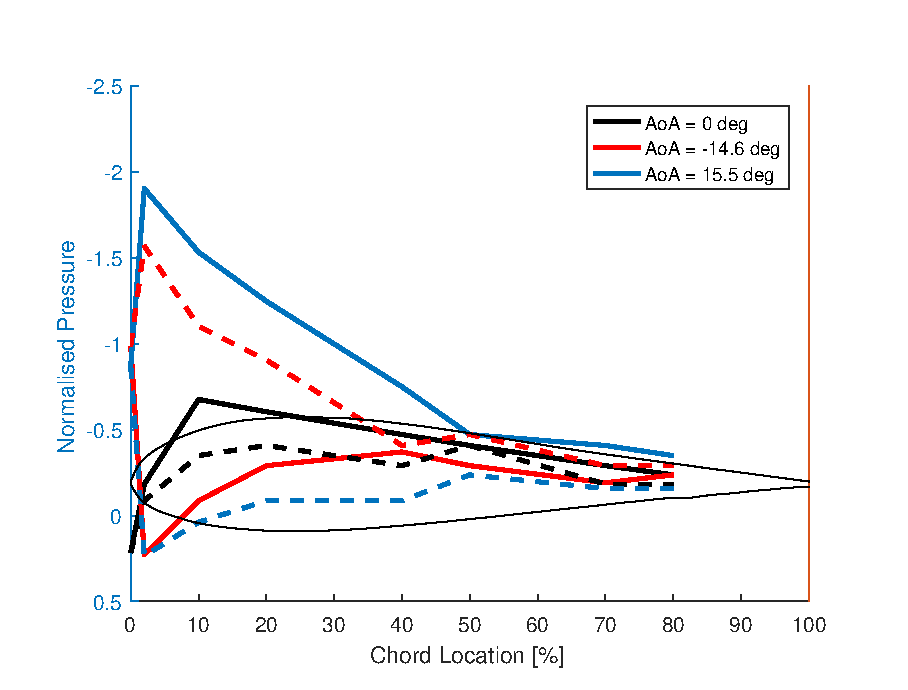
\includegraphics[height=0.6\textwidth]{PressureCoeffDistribution.eps}
				\caption{Chord-wise Normalised Pressure}
				\label{fig:CharSignals_Pressure}
      \end{figure}
		\end{column}
    \begin{column}{0.5\textwidth}
		  \begin{figure}[!htb]
        \centering
				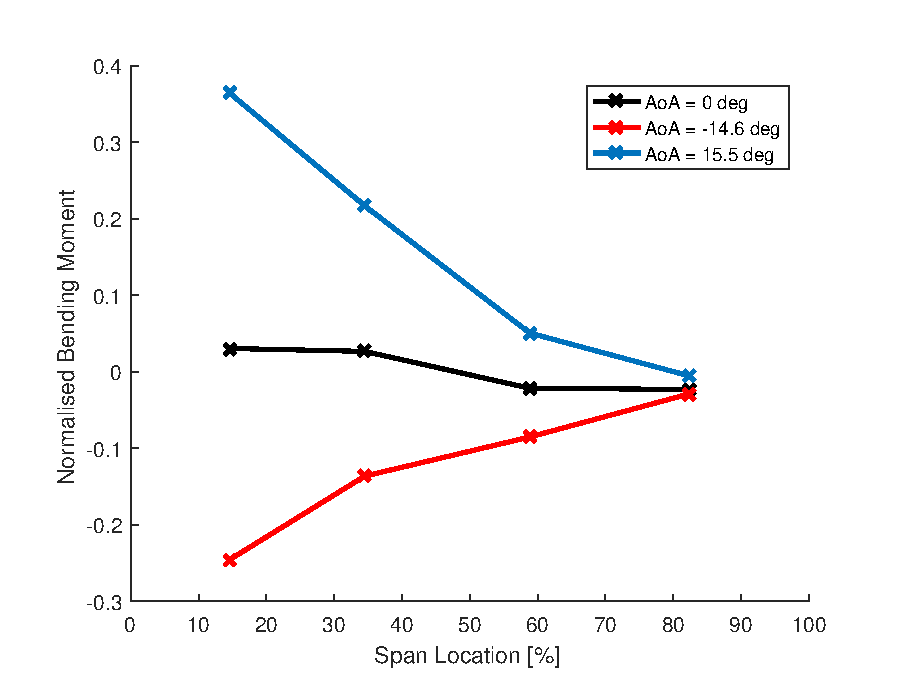
\includegraphics[height=0.6\textwidth]{BendingMomentDistribution.eps}
				\caption{Span-wise Normalised Bending Moment}
				\label{fig:CharSignals_Bending}
      \end{figure}
		\end{column}
	\end{columns}

\end{frame}

%%%%%%%%%%%%%%%%%%%%%%%%%%%%%%%%%%%%%%%%%%%%%%%%%%%%%%%%%%%%%
\begin{frame}{Current Research at UoB}

	Currently working on:
  \pause
  \begin{itemize}[<+->]
    \item{Use strain and pressure signals to}
			\begin{itemize}[<+->]
			  \item[-]{Estimated AoA, airspeed, aero-loads}
        %\item[-]{Span-wise array with 16 strain gauges}
			\end{itemize}
		\item{Design and implement closed loop control:}
			\begin{itemize}[<+->]
			  \item[-]{Classic control architecture (SISO)}
        \item[-]{Algorithm using information from distributed array, (e.g. MISO, MIMO)}
			\end{itemize}
  \end{itemize}

\end{frame}

%%%%%%%%%%%%%%%%%%%%%%%%%%%%%%%%%%%%%%%%%%%%%%%%%%%%%%%%%%%%
\section{Concluding Remarks}
\begin{frame}{Concluding Remarks}
  %What did you learn after testing?

  \pause
  \begin{itemize}[<+->]
    \item WT Characterisation experiments for strain and pressure signals
		  \begin{itemize}[<+->]
			  \item[-]{Pressure and strain signal show linear response with AoA}
        \item[-]{Stall detection potential}
				\item[-]{Strain-based roll control similar performance to IMU based control}
        \item[-]{Pitch pressure-based control similar to IMU based control}
			  \item[-]{Information not available using IMU: AoA, stall, non-linear lift}
			\end{itemize}
    %\item AoA and wind-speed ANN prediction using pressure data
  \end{itemize}
	
\end{frame}

%%%%%%%%%%%%%%%%%%%%%%%%%%%%%%%%%%%%%%%%%%%%%%%%%%%%%%%%%%%%
\section{Further Work}
\begin{frame}{Further Work}
  %What will you do with your findings next?
  %How will you further your research/findings?

  \pause
  \begin{itemize}[<+->]
    \item Phase 1: Wind tunnel testing platform
      \begin{itemize}[<+->]
      \item[-]Design and implement closed loop control algorithms
      \item[-]Carry out closed loop wind tunnel experiments
      \end{itemize}
	
    \item Phase 2: Flying platform
      \begin{itemize}[<+->]
			\item[-]Build and instrument flying platform
      \item[-]Wind tunnel experiments
      \item[-]Outdoors flight tests
      \end{itemize}
  \end{itemize}
	
\end{frame}

%%%%%%%%%%%%%%%%%%%%%%%%%%%%%%%%%%%%%%%%%%%%%%%%%%%%%%%%%%%%
\begin{frame}{}

  \centering
	\Huge{Thank you}

\end{frame}

%%%%%%%%%%%%%%%%%%%%%%%%%%%%%%%%%%%%%%%%%%%%%%%%%%%%%%%%%%%%
\end{document}

%%%%%%%%%%%%%%%%%%%%%%%%%%%%%%%%%%%%%%%%%%%%%%%%%%%%%%%%%%%%%%%%%%%%%%%%%%%%%%
